% Found this:
% http://www.astro.uni-bonn.de/~wucknitz/wiki/lib/exe/fetch.php/lbg:lbw1:preamble.tex
\chapter{Long baseline observations with LOFAR}
Observations using international LOFAR baselines have obtained science quality
images with resolution 0.3$''$ and rms noise $0.15$\,mJy\,beam$^{-1}$ at
154\,MHz, see for example \cite{varenius2014}. In this chapter we will describe
the similarities and differences in the observations and subsequent processing
as compared to LOFAR imaging using shorter (NL) baselines. This chapter is
meant to serve as a reference for you who want to plan observations or
calibrate and image LOFAR data using the longest LOFAR baselines. 
\footnote{The
authors of this chapter are Eskil Varenius ({\tt eskil.varenius@chalmers.se})
and Javier Moldon ({\tt moldon@astron.nl}) with many useful contributions from the
Long baselines working group.}
%In this chapter, the term \emph{long} baselines refer to international LOFAR
%baselines (i.e. length$~1000$\,km) unless stated otherwise.
%TODO: Outline of chapter

\section{Long baseline interferometry}
%- Key differences between short- and long-baseline interferometry. Scales for LOFAR VLBI: resolution and field of view.
The prime reson to use long baselines is to obtain very high-resolution images.
Using the longest LOFAR baselines, subarcsecond imaging is possible in the HBA
band and the upper part of the LBA band, see Table \ref{tab:res}.  However, the
wide separation of stations means that each station sees a (very) different
atmosphere, which means that visibility phases are generally less well behaved
than on shorter baselines looking through a more similar patch of the
atmosphere. Further more, the international stations cannot share the same
clock (as the core stations do) and any offsets and drifts of the clocks will
introduce delay errors between the stations. Finally, geophysical and Earth
orientation effects are more important.

\begin{table}[h]
\centering
\begin{tabular}{cccc}
Freq. & $\lambda$ & Int. station beam FWHM & Int. synthesized PSF FWHM\\
(MHz) & (m) & (deg) & ($''$)\\
\hline
15  &  20.0 &  19.39& 3.30 \\
30  &  10.0 &  9.70&   1.65\\
45  &  6.67 &  6.46&   1.10\\
60  &  5.00 &  4.85&   0.83 \\
75  &  4.00 &  3.88&   0.66\\
120 &  2.50 &  2.59&   0.41\\
150 &  2.00 &  2.07&   0.33\\
180 &  1.67 &  1.73&   0.28\\
200 &  1.50 &  1.55&   0.25\\
210 &  1.43 &  1.48&   0.24\\
240 &  1.25 &  1.29&   0.21
\end{tabular}
\caption{Values from \cite{vanhaarlem2013}.
\label{tab:res}}
\end{table}

In addition, the field of view is at long baselines not limited by the primary
beam of the largest station. Rather, the field of view is limited by the time
and frequency resolution of the data.  Since correlators output a discrete set
of visibilities (i.e. samples in time and frequency), averaging is to some
extent always done on interferometric data. We may also average the data
further after correlation to reduce the computational resources needed for
calibration and imaging. Any averaging must however be done with care.
Averaging a range of samples in time and frequency together corresponds to
averaging over a small parallelogram in Fourier space. This means some
information is lost, and one has to take care to not lose information that
could affect the scientific results.
This effect is however not only challenging, it also makes calibration
of long baseline data simpler. 
%TODO: EXPAND WITH GOOD FORMULA FOR LONG BASELINES
% TODO: With good formula, prove that since the FoV is very limited, only one
% calibration solution is necessary i.e. no multi-directional calibration is required.
% Also point out that the averaging limits the impact of interferring sources,
% thereby making the calibration easier since no demixing e.t.c. is necessary.
%TODO: Also perhaps mention phasing up the core, as a calibration thing which
% may limite the field of view.

Because of these differences, a somewhat different calibration strategy is
usually required when imaging long baseline data than what is commonly used for
LOFAR observations with shorter baselines. This need is nothing fundamentally
new for LOFAR, in fact we may borrow many tools and knowledge developed for
decades for use in very long baseline interferometry (VLBI) at centimeter
wavelengths.

\subsection{Calibration of international LOFAR stations}
%- Description of variables relevant for long baseline interferometry: phase, delay, delay rate.
%- Impact of baseline separation, ionosphere, and source structure on the phase behavior.
%- Calibrators needed in a typical long baseline observation (Dutch array calibrator, primary and secondary calibrators).
%- Differences between cm-VLBI and m-VLBI. To understand the dispersive delay produced by the ionosphere.
Data on long baselines are fundamentally no different from data on short
baselines: calibration means to correct any errors in the visibility amplitudes
and phases which were not included in the model applied when the data were
correlated (such as atmospheric effects).  If your target is very bright, you
may be able to calibrate your data using the target itself.  However, to find
amplitude and phase corrections for the international stations, the target must
be sufficiently bright on the angular scales measured by the baselines to the
international stations.  Because of the high resolution, calibration needs to
be done using either a very compact source so that a point source model is good
enough, or we need a very detailed model of the source structure. A science
target is usually both weak and potentially has complex structure (on
subarcsecond scales), which makes it hard to use for calibration of the
international stations. Therefore, a nearby bright (and preferably compact)
sources is usually observed along with the target. The amplitude and phase
errors are derived using the calibrator, and the corrections are then applied
to the target before imaging. This is called phase-referencing, and in ordinary
VLBI observations it is usually done by switching back and forth between target
and calibrator since an ordinary dish can only point in a single direction at
once. For ordinary VLBI observations this requires switching often enough so
that the corrections derived for the calibrator is valid also when observing
the target source, but since LOFAR provides multiple beams, we may observe the
calibrator and target simultaneously, simplifying calibration compared to
ordinary VLBI. However, the calibrator must also be close enough to the target 
for the corrections derived to be valid also in the direction of the target.
Preliminary investigations indicate that the separation between calibrator
and target should not be larger than 5$^\circ$, preferably closer than 1$^\circ$.
From Chapter 29. in \cite{NRAO} the isoplanatic patch size is given as 3-4$^\circ$
at 4\,m wavelength.

Finding a strong, compact (or a subarcsecond resolution modelled) calibrator within
1$^\circ$ is challenging, mainly because the sky is largely unknown at LOFAR
frequencies. Efforts are under way to build catalogues of suitable sources at
LOFAR frequencies, but often a good first guess can be found by looking at the
VLBI catalogue at higher frequencies: http://astrogeo.org/calib/search.html.
Often one have to settle for a calibrator which is compact and near the target
but which is not bright enough to calibrate the phase and amplitude separately
for each visibility (i.e. each channel/integration time).  The obvious solution
to increas the signal-to-noise (SNR) is to average the data. For shorter
baselines, one may usually average several channels and time bins together,
provided that the errors because of e.g. the atmosphere does not introduce
phase or amplitude changes within the averaging interval. However, for long
baselines the errors are more serious, for example because of the very
different atmospheres above the stations. The ionosphere may introduce
\emph{delay} errors (phase slope vs. frequency) of several hundred nanoseconds,
which means that the visibility phases will change several cycles within a few
MHz of LOFAR data. Blindly averaging such data will severely reduce the
amplitude of the calibrator signal. If the phase also changes with time there
will be a phase slope vs. time as well, which is referred to as a fringe
\emph{rate}.  This means that simple averaging cannot be done to increase the
SNR. This is usually the case also in cm-VLBI, and to be able to use the weaker
calibrators the VLBI community has developed a technique usually referred to as
\emph{fringe fitting}. 
Global fringe fitting solving for delays and rates is, when writing this,
only available within the Astronomical Image Processing System (AIPS,
see http://www.aips.nrao.edu). To read the data into AIPS, we first need
to convert from the standard LOFAR format of Measurement sets in alinear (X,Y)
polarisation basis to UVFITS-files in a circular (R,L) polarisation basis. 
This is done in two steps, first the conversion to circular and then the conversion
to UVFITS.

\subsection{Conversion to circular polarisation basis}
%- To understand why circular polarization is useful and how to convert the data.
Standard VLBI techniques like fringe fitting work in a circular (R,L)
polarisation basis. In this basis, the ionospheric disturbances are transformed
from coupled amplitude/phase effects (as in the linear X,Y basis) to phase only 
effects. Also, since differential Faraday rotation does not mix R and L
polarisations we may calibrate RR and LL independently. Conversion to 
circular polarisation may be done using different tools. 
The M82 data \cite{varenius2014} were converted from linear to circular
using the tool \emph{mscorpol} v1.6, developed by T. D. Carozzi.
This tool includes corrections for dipole-projection effects as a function of
the correlated sky position relative to all included LOFAR stations.  After the conversion,
the data are circularly polarised, with full (but approximated) parallactic angle
correction. 

\subsection{The UV-FITS format}
%- Brief introduction + references to FITS files, convert them, and manipulate them in AIPS.
Since AIPS understands the UVFITS-format, but not Measurement Sets (MS)
we need to convert the data from MS to UVFITS. There are several ways to do this:
\begin{itemize}
\item You may use the function \emph{exportuvfits} in CASA.
\item You may use the tool \emph{ms2uvfits} available at the LOFAR cluster, as {\tt ms2uvfits in=[input-MS] out=[output-FITS-file] writesyscal=False}
\end{itemize}

\subsection{Loading the data into AIPS}
The AIPS task FITLD can be used to load the data in to AIPS. For LOFAR data,
the parameters digicor=-1 and douvcomp=-1 should used.

\section{Fringe fitting}
%- How to conduct a VLBI phase calibration in AIPS (FRING)
%- Inspection of phase solutions and to understand their meaning.
The precedure used to find and correct residual rates and delays is called
\emph{fringe fitting}. A fringe fit is nothing more than a self-calibration
including not only phases and amplitudes, but also derivatives of the phase
with respect to frequency and time.  By doing this, more data can be included
in the fitting process thereby increasing the signal-to-noise, which enables
solutions to be found for weak sources and/or in noisy data. In AIPS the most
commonly used task for this is called \verb!FRING!. This task considers the
first derivatives of phase vs. frequency and time, i.e. it assumes linear
delays and rates within the selected bandwidth and solution interval.  

%TODO: CURVATURE 

As an example, let's inspect two minutes of data on a particular baseline
(CS001HBA - DE601HBA) for the source J0958+6533, the source used to find and
correct residual delays and rates by \cite{varenius2014}.  The raw-data is
plotted using the AIPS task \verb!POSSM!  in Fig. \ref{fig:J0958Hprefring}.
From this figure we can see by eye that the phase $\phi$ changes approximately
$\Delta \phi=1.5$ cycles (i.e.  $1.5\cdot2\pi$ radians) over the full bandwidth
of $\Delta \nu=$15.9\,MHz.  Assuming a linear phase gradient we can estimate
the delay as $\tau = \Delta \phi / \Delta \nu=94$\,ns at this particular time.
Indeed, FRING finds a very similar value as can be seen around 22 UT in
\ref{fig:J0958Hdelays}.  These corrections were found using the default parameters of FRING,
with the following manual changes: The search was restricted to baselines longer than 60k$\lambda$ (\verb!uvrange = 60,0!), 
a delay search window of 600\,ns (\verb!dparm[2]=600!), a rate search window of 30\,mHz (\verb!dparm[3]=30!), and a solution interval of
2 minutes (\verb!solint=2!).  Solutions were found separately for each IF and polarisation.

After applying the corrections from FRING, the phase
is flat with respect to frequency, see \subref{fig:J0958Hpostfring}, as it
should be for a point source.

\begin{figure*}[htbp]
\centering
\subfigure[Before fringe fitting]{
    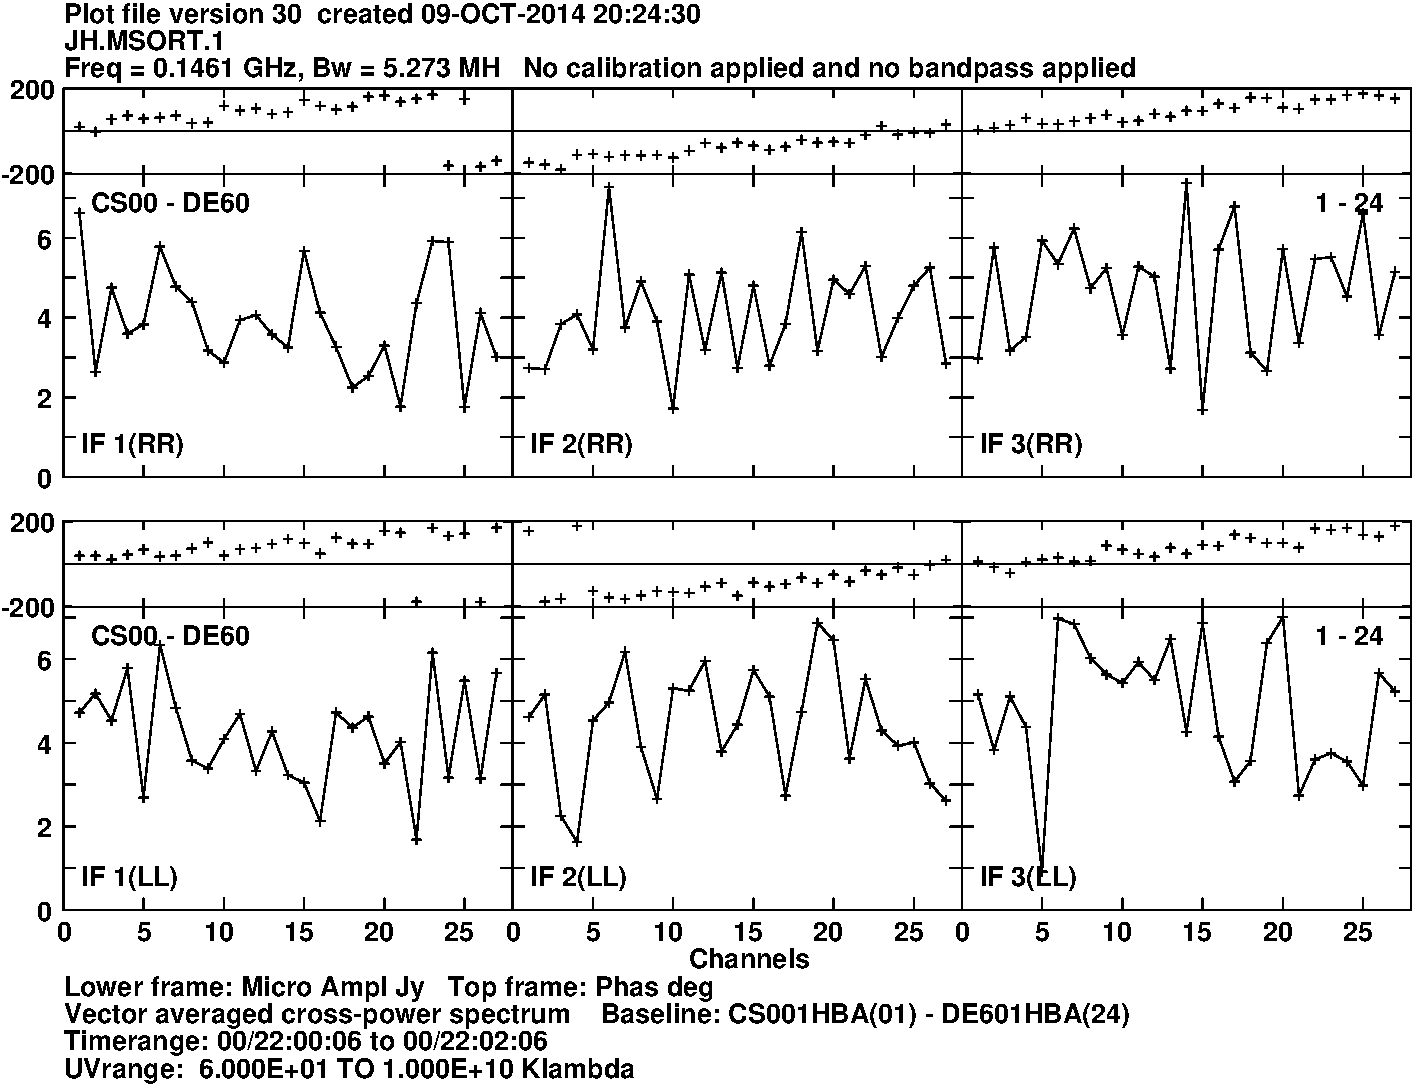
\includegraphics[width=0.8\textwidth]{figs/J0958Hprefring-crop.pdf}
    \label{fig:J0958Hprefring}
}
\subfigure[After fringe fitting]{
    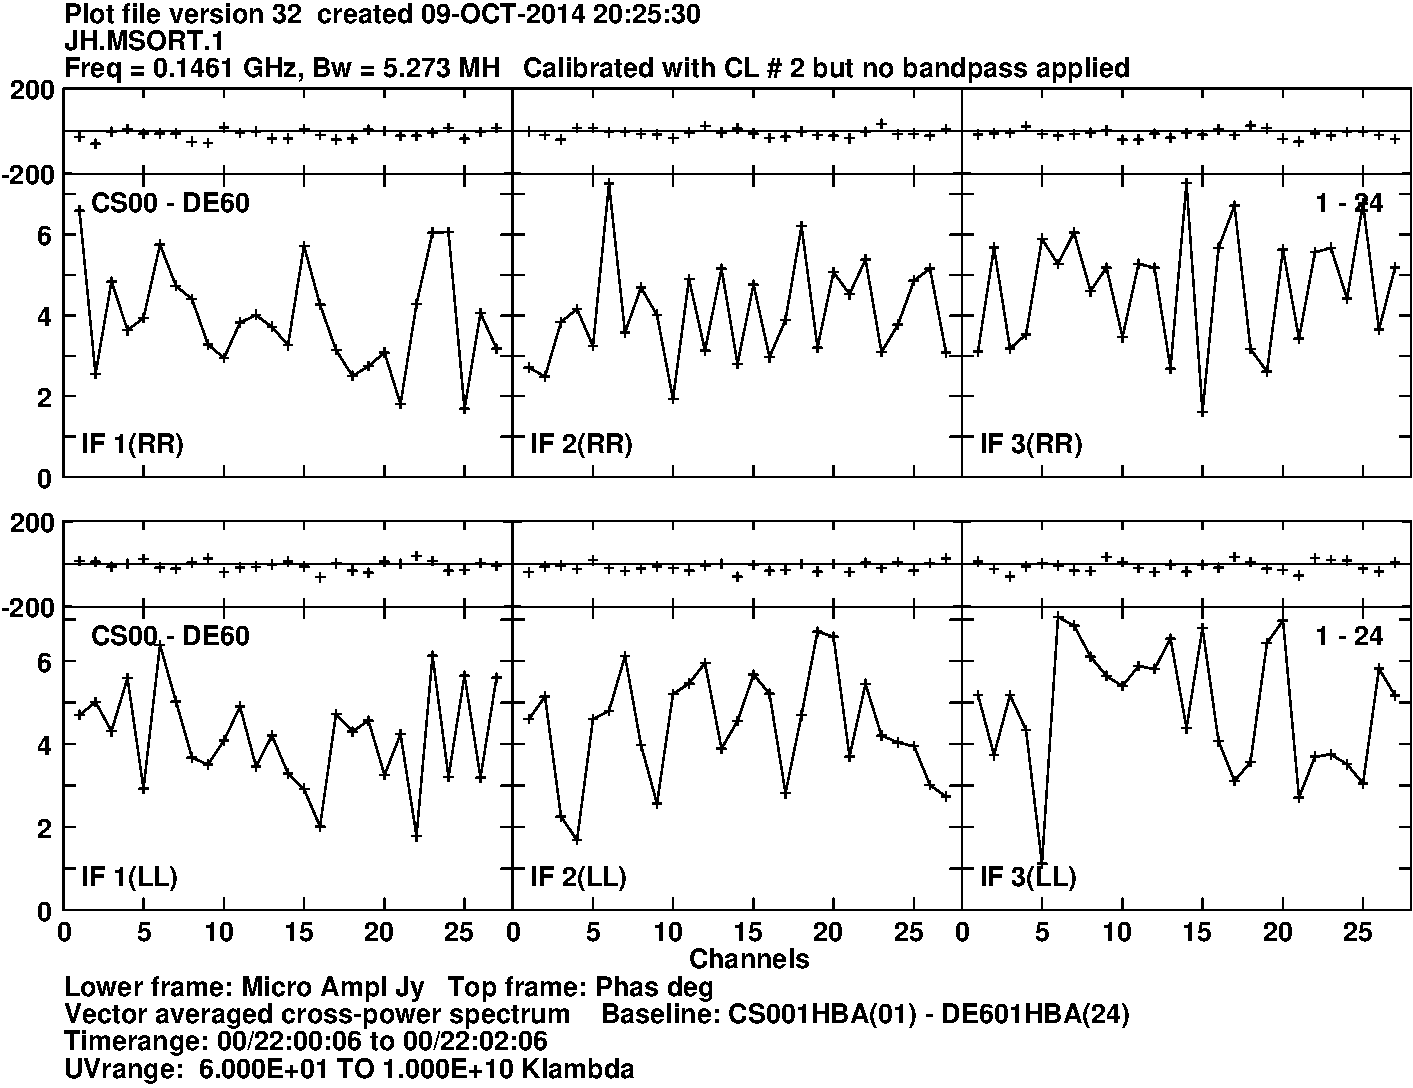
\includegraphics[width=0.8\textwidth]{figs/J0958Hpostfring-crop.pdf}
    \label{fig:J0958Hpostfring}
}
\caption{
Two figures showing the effect of fringe fitting on two minutes of data on the baseline CS001HBA - DE601HBA. Both 
polarisations are shown, and the data are divided in three spectral windows (IFs in AIPS) of 5.3\,MHz each. 
After applying the corrections from FRING,
the phase is flat with respect to frequency, see \subref{fig:J0958Hpostfring}, as it should be for a point source.
\label{fig:fringex}
}
\end{figure*}

\begin{figure*}[htbp]
\centering
\subfigure[Delay corrections for DE601HBA IF2]{
    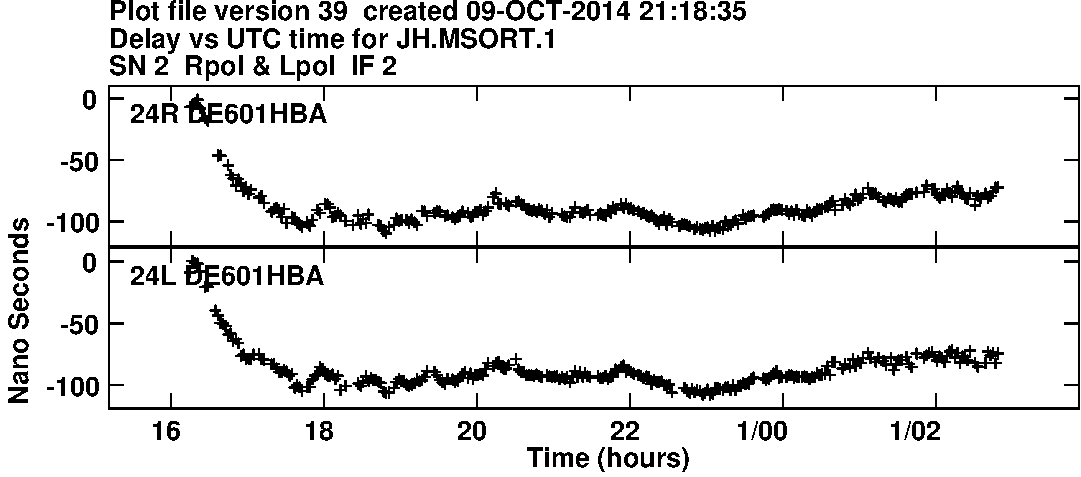
\includegraphics[width=0.8\textwidth]{figs/J0958Hdelays-crop.pdf}
    \label{fig:J0958Hdelays}
}
\subfigure[Rate corrections for DE601HBA IF2]{
    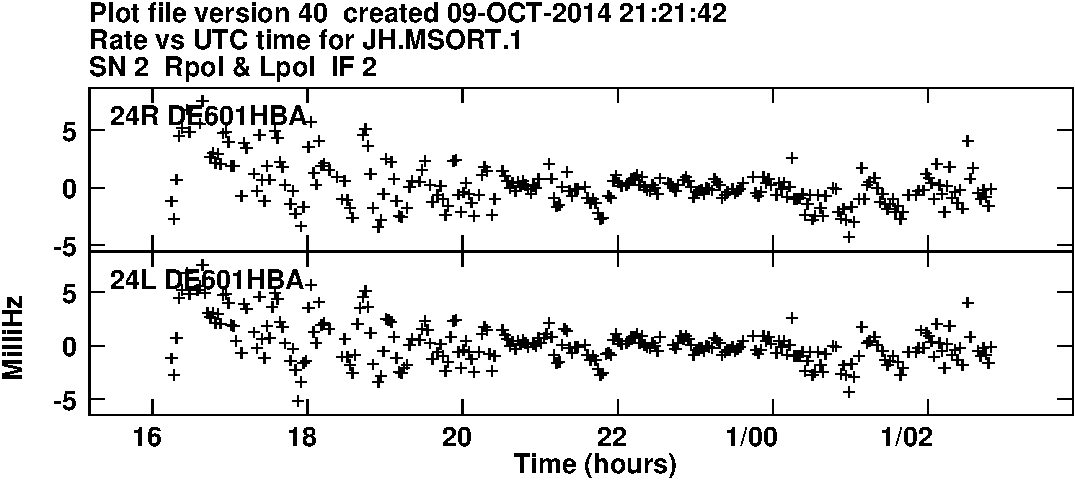
\includegraphics[width=0.8\textwidth]{figs/J0958Hrates-crop.pdf}
    \label{fig:J0958Hrates}
}
\subfigure[Phase corrections for DE601HBA IF2]{
    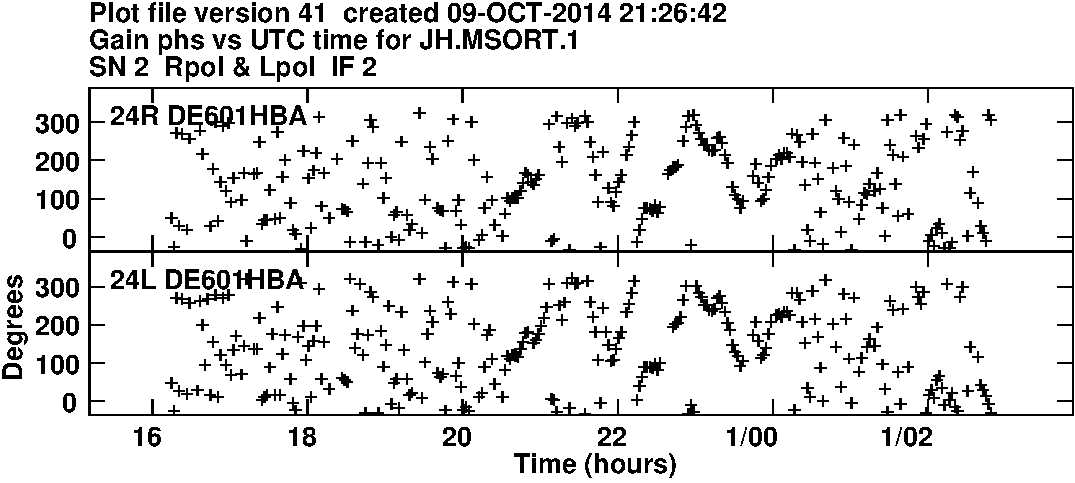
\includegraphics[width=0.8\textwidth]{figs/J0958Hfringpsol-crop.pdf}
    \label{fig:J0958Hfringphases}
}
\caption{
Delay (\subref{fig:J0958Hdelays}), rate (\subref{fig:J0958Hrates}) and phase
\subref{fig:J0958Hfringphases} corrections derived for the source J0958 at 154\,MHz
by FRING for antenna DE601HBA.  These plots show the corrections derived for
the whole 10 hour observation (the first segment of project LC0\_026). It is
clear from the rates and phases that phases changes rapidly during the first
and last hours of the experiment. The delay solutions are more stable, although
there is a large change in at the start. In general, the ionosphere is more
stable during midnight than at sunset or sunrise. 
}
\label{fig:fringsols}
\end{figure*}
Inspect the solutions carefully with SNPLT after use of FRING. The
solutions should be smoothly varying with time, and are typically a
few tens of nanoseconds for most antennas. Large delays (microseconds
or above) should be reported to the Observatory, particularly if they
appear in more than one dataset or if there are sudden changes in
the delay.

\subsection{Applying the solutions}
Describe optinally SNSMO, CLCAL.

\subsection{Amplitude calibration}
%- Ways to obtain the amplitude calibration for international stations
As described in Sect. X, the calibrator used for deriving delay, rate and phase
corrections need to be close to the target and sufficiently compact to show
enough signal on the longest baselines. This calibrator can in principle also
be used for amplitude calibration of the long baselines, but again a good model
is required. For fringe finding, the only requirement for good solutions is
that the calibrator is bright enough and compact enough.  But, for amplitude
calibration, we must know the flux density of the calibrator.  Usually the VLBI
calibrators stay compact, but the flux density can vary more than a factor of
two between observations due to intrinsic variability. Therefore they cannot be
trusted to set the amplitude scale of the observation. 

For the case of M82, the calibrator J0958 is bright and compact enough for amplitude
calibration of the international baselines, but we did not know the correct flux density. 
Therefore, we included observations also of a known flux calibrator, 3C196. Now, the calibrator J0958
was used to track possible amplitude variations during the observation for all stations, and
3C196 was used to check the absolute amplitude scale, i.e. to find the flux density of J0958. 

The amplitude corrections should be smooth, and will in most cases show a larger gain at the start and end of an experiment.
This is because an observation is usually centered in time so that the target will reach its peak elevation at the middle of the
observation time. This means that it will be at lower elevation in the begining and end of the observation, which means that
the projected station area will be less at the start and end times. This in turn means that the sensitivity is lower at the start
and end times, which means that the gain corrections need to be larger (and will be noisier) at these times. As an example,
let us look at the gain corrections derived by CALIB in AIPS for DE601HBA on J0958, see Fig. \ref{fig:ampcal}.
When running CALIB, we have decreased the number of free parameters compared to FRING, since we are now only solving for amplitude and phase. 
It is therefore possible to find minor phase corrections at this point which was not perfectly determined by FRING.

\begin{figure*}[htbp]
\centering
\subfigure[Amplitude corrections for DE601HBA IF2]{
    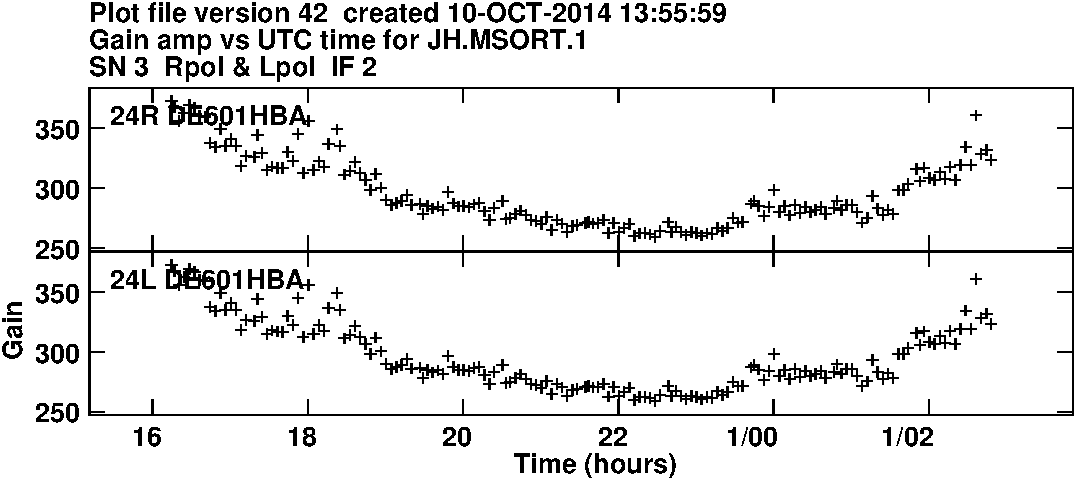
\includegraphics[width=0.8\textwidth]{figs/J0958Hampsols-crop.pdf}
    \label{fig:J0958Hamps}
}
\subfigure[Phase corrections for DE601HBA IF2]{
    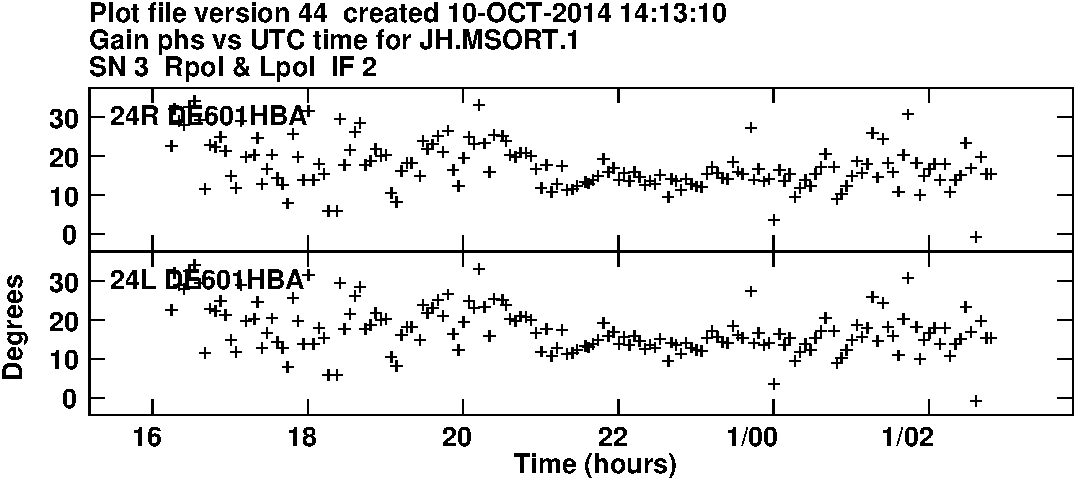
\includegraphics[width=0.8\textwidth]{figs/J0958Hphase-crop.pdf}
    \label{fig:J0958Hphases}
}
\caption{
The amplitude and phase corrections derived by CALIB for the international LOFAR station DE601HBA during the first 10 hours of project LC0\_026. 
We see larger, and more noisy, corrections at the beginning and end of the experiment, as expected from the smaller
projected station area at these times relative to transit. 
\label{fig:ampcal}
}
\end{figure*}
    
The final result of calibration for this baseline can be seen in Fig. \ref{fig:vplot}.
\begin{figure*}[htbp]
\centering
    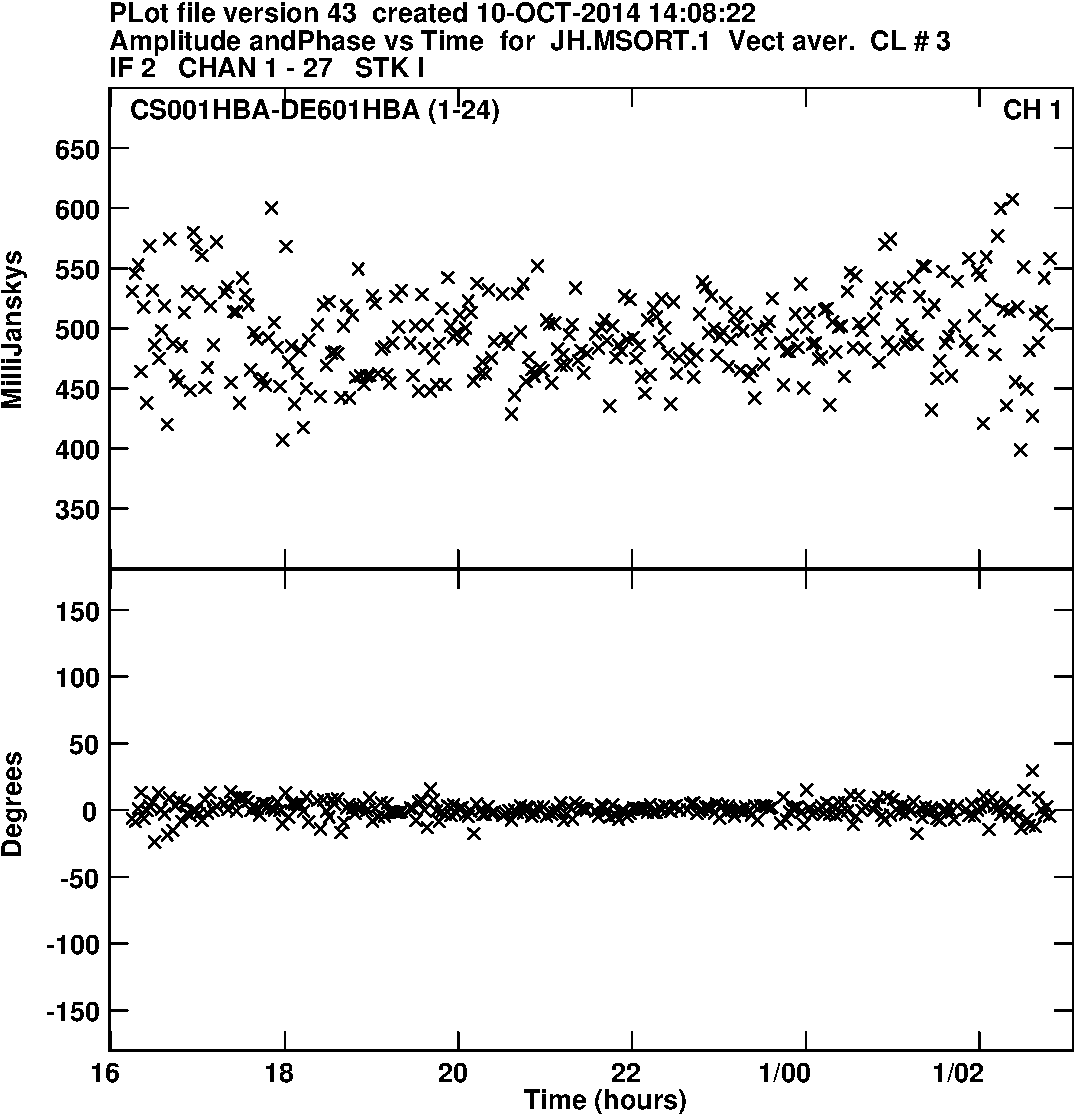
\includegraphics[width=0.8\textwidth]{figs/J0958Hvplot-crop.pdf}
\caption{
The final visibility amplitudes and phases on the DE601HBA-core baseline. We assumed this source to be a 0.5Jy point source, which means that we should now see two straight lines
in this plot: one for the amplitude centered at 500\,mJy, and one for the phase centered at 0 degrees. This is also what we see using VPLOT in AIPS to inspect the data. Apart from noise,
there are marginal changes differences to a point source. It is clear from \cite{varenius2014} that this object has a weak extension to the south-west, and this should create 
minor deviations in the visibilites compared to those of a point source.
\label{fig:vplot}
}
\end{figure*}

\subsection{High-resolution imaging}
%- Brief comments on high-resolution imaging.
Although AIPS can determine delays and rates, it is not the best option for imaging long baseline LOFAR data. Since we consider asmall field of view, we do not need 
the beam models offered by AW-imager. However, at subarcsecond resolution we will may need to take into account any effects of a non-coplanar array, i.e. W-projection. The field of view $\theta_\mathrm{f}$
possible to image without W-projection (i.e. using a single tangent plane) can be estimated as $\theta_{\mathrm{f}} = \sqrt{\theta_{\mathrm{b}}}/3$ (see 2-29 in \cite{NRAO}) where $\theta_\mathrm{b}$
is the FWHM of the synthesized beam, both $\theta$ in radians. If your field of view is larger than this you need to perform deconvolution using W-projection, for example in CASA.

\subsection{Combining the core into a single superstation}
%- How to form a sensitive tied station from the LOFAR core stations.
TODO: This section chould include parset files, background info about strong
calibrator and also plot of the station beam producet by the phased up core.
Eskil's calculations at 154MHz suggest 5\% amplitude loss at 30$''$ distance
from phase center, which is the most serious of all effects mentioned in this
document regarding field of view. Also, it is not clear to me if NDPPP
phase-rotates the data properly when adding the beams in a specific direction,
if using the shift-average approach in the coming pipeline.

